\documentclass[letterpaper]{article}
\usepackage[utf8]{inputenc}
\usepackage[spanish, mexico]{babel}
\usepackage{amssymb, amsmath}
\usepackage{graphicx}
\usepackage[margin=1.5cm,
vmargin={1.5cm,0.7cm},
includefoot]{geometry}
\usepackage{amsthm}
\usepackage{dsfont}
\usepackage{mathtools}
\usepackage{graphicx}
\usepackage{algorithmic}
\usepackage[linesnumbered,ruled,vlined]{algorithm2e}
\begin{document}

\setlength{\unitlength}{1cm}
\thispagestyle{empty}
\begin{picture}(19,3)
\put(-0.5,1.2){
\includegraphics[scale=.20]{img/unam1.png}}
\put(16,1){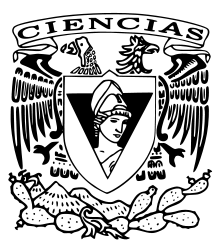
\includegraphics[scale=.29]{img/fciencias1.png}}
\end{picture}

\begin{center}
	\vspace{-114pt}
	\textbf{\large Proyecto 01}\\
	\textbf{ Semestre 2021-1}\\
	Prof. José Galaviz Casas\\
	Ayud. María Ximena Lezama \\
	\textbf{Modelado y programación}\\[0.15cm]
	Kevin Ariel Merino Peña\footnote{Número de cuenta 317031326} Armando Abraham Aquino Chapa\footnote{Número de cuenta n}\\
	\today
\end{center}
\vspace{-10pt}
\rule{19cm}{0.3mm}

\section{Definición del problema}
\section{Análisis del problema}
	\textbf{Análisis del problema y selección de la mejor alternativa. }
	Al ir analizando los diversos rubros que puede abarcar el problema, se determinó que lo más adecuado para resolverlo era obtener las siguientes clases:
	\begin{itemize}
		\item \textbf{Clase Weather:}.
		\begin{itemize}
			\item Esta clase sería la encargada de realizar las distintas peticiones al servidor para obtener todos los datos correspondientes al clima.
			\item Manejar los posibles errores, como el exceso de numero peticiones en un lapso de tiempo, para no obtener ningún problema con el servidor,y manejar los errores donde no es posible consultar la información
			\item Otorgar de un formato correcto y legible a la salida del programa
		\end{itemize}
		\item \textbf{Clase CSVReader}
		\begin{itemize}
			\item Su función principal sería leer los archivos \textit{csv} otorgados por el aeropuerto de la Ciudad de México.  
			\item Preprocesar cierto tipo de información que si es esencial de la que es redundante o no tiene utilidad para nuestros objetivos.
			\item
			
		\end{itemize}
	\end{itemize}
	
\section{Selección de la mejor alternativa}

\section{Pseudocódigo}

	\subsection*{CSVReader.py}
	
	\begin{algorithm}
		\SetKwData{Left}{left}\SetKwData{This}{this}
		\SetKwData{Up}{up}
		\SetKwFunction{Union}{Union}
		\SetKwFunction{FindCompress}{FindCompress}
		\SetKwInOut{Input}{Entrada}
		\SetKwInOut{Output}{Salida}
		\SetAlgorithmName{Función}{0}{list of algorithms name}
		\Input{Nombre de un archivo (ruta)}
		\Output{Lista de coordenadas no repetidas}
		\BlankLine
		\While{Archivo(nombre dado) esté abierto}{
		\ForEach{renglones $\leftarrow$ documento}{
				\If{(latitud , longitud ) \textbf{no} están en  la lista}{
				Agreagrlas}
		}
	}
	\caption{read\_no\_repeated\_coordinates}
	\end{algorithm}
	
	\begin{algorithm}
		\SetKwData{Left}{left}\SetKwData{This}{this}
		\SetKwData{Up}{up}
		\SetKwFunction{Union}{Union}
		\SetKwFunction{FindCompress}{FindCompress}
		\SetKwInOut{Input}{Entrada}
		\SetKwInOut{Output}{Salida}
		\SetKwProg{try}{try}{:}{}
		\SetKwProg{catch}{catch}{:}{end}
		\SetAlgorithmName{Función}{0}{list of algorithms name}
		\Input{Nombre de un archivo (ruta)}
		\Output{Lista de diccionarios con vuelos}
		\BlankLine
		\try{}{
				Abrir ruta\\
				\For{linea $ \gets $ archivo}{
				linea $ \gets $ lista}
		}
		\catch{FileNotFoundError}{
			\textbf{muesta}	 Error, escribe una ruta válida\\\textbf{exit}
		}
		\catch{FileExistsError}{
		\textbf{muesta}	 Error, archivo válido\\\textbf{exit}
		}
	\caption{read\_csv\_file}
	\end{algorithm}
	
	\begin{algorithm}
		\SetKwData{Left}{left}\SetKwData{This}{this}
		\SetKwData{Up}{up}
		\SetKwFunction{Union}{Union}
		\SetKwFunction{FindCompress}{FindCompress}
		\SetKwInOut{Input}{Entrada}
		\SetKwInOut{Output}{Salida}
		\SetKwProg{with}{with}{:}{}
		\SetKwProg{catch}{catch}{:}{end}
		\SetAlgorithmName{Función}{0}{list of algorithms name}
		\Input{Nombre de un archivo (ruta)}
		\Output{Lista de cabeceras}
		\BlankLine
		\with{}{
			lector $ \gets $ \textbf{Leer primera linea}( ruta)
		}
	\caption{read\_headers}
	\end{algorithm}
	\newpage
	\subsection*{main.py}
	
	\begin{algorithm}
		\SetKwData{Left}{left}\SetKwData{This}{this}
		\SetKwData{Up}{up}
		\SetKwFunction{longitud}{longitud}
		\SetKwFunction{vf}{validate\_file}
		\SetKwFunction{readHeaders}{read\_headers}
		\SetKwInOut{Input}{Entrada}
		\SetKwInOut{Output}{Salida}
		\SetKwProg{with}{with}{:}{}
		\SetKwProg{catch}{catch}{:}{end}
		\SetAlgorithmName{Función}{0}{list of algorithms name}
		\Input{Nombre de un archivo (ruta) pasados como argumento al programa}
		\BlankLine
		\If{longiutd del argumento no es 2}{
		\textbf{muestra:} Error \\Debe indicar la ruta a un archivo csv\\ \textbf{salir}}
		\If{no coincide la extensión .csv}{\textbf{muestra: } Error, sólo admito archivos csv \\\textbf{salir}}
		cabezera $ \gets $ nombres de listas admitidas\\
		entrada\_cabecera $ \gets $ \readHeaders{argumento[1]}{}\\
		\If{\longitud{entrada\_cabecera} no es igual a \longitud{cabezera}}{
		\textbf{muestra:} ERROR El archivo csv debe tener los siguientes encabezados: origin, destination, origin\_latitude, origin\_longitude, destination\_latitude, destination\_longitude \\
		\textbf{salir}}
		\ForEach{cabeza in entrada\_cabezera}{\If{cabeza no está en cabezera}{\textbf{muestra:} ERROR El archivo csv debe tener los siguientes encabezados: origin, destination, origin\_latitude, origin\_longitude, destination\_latitude, destination\_longitude\\ \textbf{salir} }}
	\caption{validate\_file}
	\end{algorithm}
	
	\begin{algorithm}
		\SetKwData{Left}{left}\SetKwData{This}{this}
		\SetKwData{Up}{up}
		\SetKwFunction{makeapirequestbycoordinates}{make\_api\_request\_by\_coordinates}
		\SetKwFunction{format}{format}
		\SetKwFunction{setdefault}{setdefault}
		\SetKwFunction{vf}{validate\_file}
		\SetKwFunction{readcsvfile}{read\_csv\_file}
		\SetKwFunction{readnorepeatedcoordinates}{read\_no\_repeated\_coordinates}
		\SetKwInOut{Input}{Entrada}
		\SetKwInOut{Output}{Salida}
		\SetKwProg{with}{with}{:}{}
		\SetKwProg{catch}{catch}{:}{end}
		\SetAlgorithmName{Función}{0}{list of algorithms name}
		\Input{Nombre de un archivo (ruta)}
		\BlankLine
		%%%%%%%%%%%%%%%%%%%%%%%%%%%%%%
		\vf{argumentos al correr el programa}{}\;
		entradas $ \gets $ \readcsvfile{argumento al correr el programa}\\
		%%%%%%%5
		solicitudes\_no\_repetidas $ \gets $ \readnorepeatedcoordinates{argumentos al iniciar}\\
		\ForEach{solicitud \textbf{en} solicitudes\_no\_repetidas}{
		peticion $ \gets $ \makeapirequestbycoordinates{solicitud[0], solicitud[1]}\\
		peticiones $ \gets $ \setdefault{solicitud, peticion}\\
		}	
		\ForEach{entrada \textbf{en} entradas}{\textbf{muesta: } Datos del clima ;) con formato bonito }
	\caption{run}
	\end{algorithm}
	
	\newpage
	\subsection*{Weather.py}
	\begin{algorithm}
		\SetKwData{Left}{left}\SetKwData{This}{this}
		\SetKwData{Up}{up}
		\SetKwFunction{makeapirequestbycoordinates}{make\_api\_request\_by\_coordinates}
		\SetKwFunction{get}{get}
		\SetKwInOut{Input}{Entrada}
		\SetKwInOut{Output}{Salida}
		\SetKwProg{with}{with}{:}{}
		\SetKwProg{catch}{catch}{:}{end}
		\SetAlgorithmName{Función}{0}{list of algorithms name}
		\Input{latitud, lontigud}
		\Output{llamada a función parse\_weather\_info }
		\BlankLine
		%%%%%%%%%%%%%%%%%%%%%%%%%%%%%%
		\If{contador $ > $ 59}{contador $ \gets $ 0\\ esperar 1 minuto para continuar}
		\get{url + latitud y longitud dadas}{}\\
		contador $ \gets $ contador + 1
	\caption{make\_api\_request\_by \_coordinates}
	\end{algorithm}
	
	\begin{algorithm}
		\SetKwData{Left}{left}\SetKwData{This}{this}
		\SetKwData{Up}{up}
		\SetKwFunction{getLocalzone}{get\_localzone()}
		\SetKwFunction{fromTimeStamp}{fromtimestamp}
		\SetKwFunction{strftime}{strftime}
		\SetKwInOut{Input}{Entrada}
		\SetKwInOut{Output}{Salida}
		\SetAlgorithmName{Función}{0}{list of algorithms name}
		\Input{Número de fecha y hora (unix)}
		\Output{cadena de texto con hora en formato 12 hrs}
		\BlankLine
		%%%%%%%%%%%%%%%%%%%%%%%%%%%%%%
		\textbf{convierte\_fotante: } numero dado\\
		local\_timezone $ \gets $ \getLocalzone{ }\\
		local\_time $ \gets $ \fromTimeStamp{flotante, local\_timezone}\\
		\textbf{regresar: } local\_time con formato de 12 horas, (CODIGO DEL TIEMPO)
	\caption{formato\_de\_horas}
	\end{algorithm}
	
	\begin{algorithm}
		\SetKwData{Left}{left}\SetKwData{This}{this}
		\SetKwData{Up}{up}
		\SetKwFunction{makeapirequestbycoordinates}{make\_api\_request\_by\_coordinates}
		\SetKwFunction{get}{get}
		\SetKwInOut{Input}{Entrada}
		\SetKwInOut{Output}{Salida}
		\SetKwProg{try}{try}{:}{}
		\SetKwProg{catch}{catch}{:}{end}
		\SetAlgorithmName{Función}{0}{list of algorithms name}
		\Input{respuesta en formato json}
		\Output{llamada a función parse\_weather\_info }
		\BlankLine
		%%%%%%%%%%%%%%%%%%%%%%%%%%%%%%
		\try{ }{
		extraer información del archivo json con las llaves proporcionadas por la documentación de la API}
		\catch{KeyError}{
		\textbf{regresar: } Error, no se pudo consultar la información}
		\textbf{regresar: } El pronóstico del clima es: X , humedad: x\\ \qquad \qquad \quad Temperatura actual: X$ ^\circ $C, mínima: X$ ^\circ $C, máxima: X$ ^\circ $C Amanecer: X Puesta del sol: X
	\caption{parse\_weather\_info}
	\end{algorithm}




\section{Mejora a futuro}
ocument}